\chapter{\centering \textbf{\MakeUppercase{Title of Some Important contents}}}
\justifying
[Small Introduction]
\section{\textbf{\MakeUppercase{Section Title}}}

The global path planning for the coverage region is defined as the path taken by the robot from a start position Ps(x, y) to an exit position Pe(x, y) while passing through all accessible places and avoiding obstacles. To get this global path, partition it into mini-paths, the latter of which must not exceed the sensor's range, as shown in Fig. 4.1.\\
\\\begin{figure}[htb]
\centering
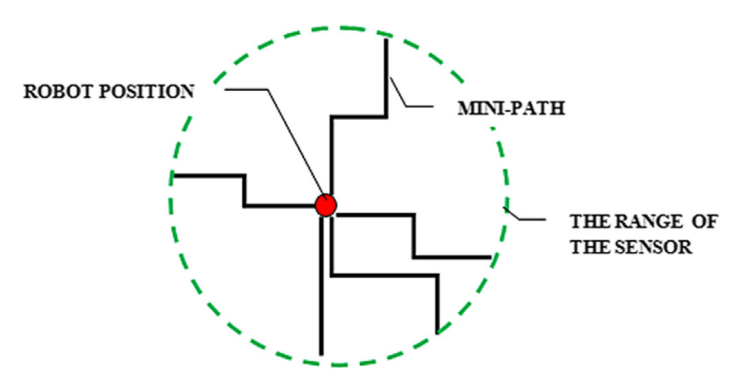
\includegraphics[scale=0.5]{fig4.1.png} % e.g. insert ./image for image.png in the working directory, adjust scale as necessary
\caption{\texttt{}The path planning method\texttt{}}
\label{fig:label} % insert suitable label, this is used to refer to a fig from within the text as shown above
\end{figure}\\

[Add your content and learn how to add images from the example  above]
